\documentclass[tikz,border=6pt]{standalone}
\usepackage{amsmath,amssymb}
\usepackage{xcolor}
\definecolor{accent}{HTML}{A13D2C}
\definecolor{accent2}{HTML}{2B5F6B}
\definecolor{muted}{HTML}{5A564F}
\definecolor{linecol}{HTML}{D8D2C4}
\definecolor{astroblue}{HTML}{1B4F72}
\usetikzlibrary{calc,arrows.meta}
\usepackage[T1]{fontenc}\usepackage{newpxtext,newpxmath}  % same fonts as the notes
\begin{document}
% x = h nu / k_B T_CMB. Blue: CMB intensity shape x^3/(e^x-1). Red: Sunyaev-Zel'dovich change of that shape per unit y,
% x^4 e^x/(e^x-1)^2 [x coth(x/2) - 4]. Both in units of 2 (k_B T_CMB)^3/(h c)^2. Null at x = 3.83.
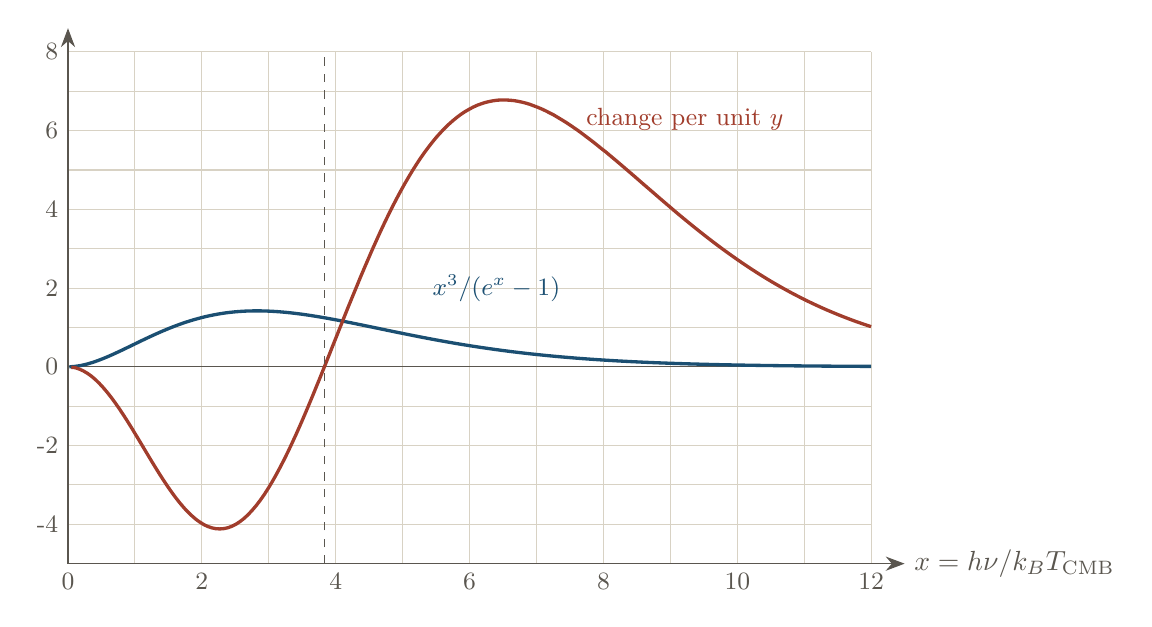
\begin{tikzpicture}[x=0.85cm,y=0.5cm, >={Stealth[length=2.4mm]}]
  \draw[linecol] (0,-5) grid[xstep=1,ystep=1] (12,8);
  \draw[muted] (0,0) -- (12,0);
  \draw[->, muted] (0,-5) -- (12.5,-5) node[right] {$x=h\nu/k_BT_{\rm CMB}$};
  \draw[->, muted] (0,-5) -- (0,8.6);
  \foreach \x in {0,2,4,6,8,10,12} \node[below, muted] at (\x,-5) {\small \x};
  \foreach \y in {-4,-2,0,2,4,6,8} \node[left, muted] at (0,\y) {\small \y};
  \draw[astroblue, line width=1.2pt, domain=0.02:12, samples=200] plot (\x, {exp(3*ln(\x)-\x)/(1-exp(-\x))});
  \draw[accent, line width=1.2pt, domain=0.05:12, samples=200] plot (\x, {exp(4*ln(\x)-\x)/(1-exp(-\x))^2*(\x*(1+exp(-\x))/(1-exp(-\x))-4)});
  \draw[dashed, muted] (3.830,-5) -- (3.830,8);
  \node[astroblue, right] at (5.3,2.0) {\small $x^3/(e^x-1)$};
  \node[accent, right] at (7.6,6.3) {\small change per unit $y$};
\end{tikzpicture}
\end{document}
